\section{Modelling and Control}
\label{sec:model}

\subsection{USV Model}

The WAM-V is described in the horizontal plane by its position $(x,y)$ and heading $\psi$ in the inertial frame, and by its surge, sway and yaw velocities $(u,v,r)$ in its body frame. The kinematics are $\dot x = u\cos\psi - v\sin\psi$, $\dot y = u\sin\psi + v\cos\psi$ and $\dot\psi = r$, and the dynamics follow from Newton's and Euler's laws in the rotating body frame, with the linear-plus-quadratic hydrodynamic damping of~\cite{fossenHandbookMarineCraft2011},
\begin{equation}
\begin{aligned}
    \dot u &= \tfrac{1}{m}\big[X - (X_u + X_{uu}^{\pm}|u|)u\big] + vr, \\
    \dot v &= \tfrac{1}{m}\big[Y - (Y_v + Y_{vv}|v|)v\big] - ur, \\
    \dot r &= \tfrac{1}{I_z}\big[N - (N_r + N_{rr}|r|)r\big],
\end{aligned}
\label{eq:usv_dyn}
\end{equation}
where the quadratic surge damping $X_{uu}^{\pm}$ differs between forward and backward motion. The forces and moment $(X,Y,N)$ are produced by two azimuth thrusters, with thrusts $T_L, T_R$ and angles $\alpha_L, \alpha_R$, mounted at $(-x_{arm}, \pm y_{arm})$,
\begin{equation}
\begin{aligned}
    X &= T_L\cos\alpha_L + T_R\cos\alpha_R, \\
    Y &= T_L\sin\alpha_L + T_R\sin\alpha_R, \\
    N &= -x_{arm}(T_L\sin\alpha_L + T_R\sin\alpha_R) \\
      &\quad - y_{arm}(T_L\cos\alpha_L - T_R\cos\alpha_R).
\end{aligned}
\label{eq:usv_alloc}
\end{equation}

\subsection{UAV Model}

The x500 is described by its position $\mathbf{p} = [x,y,z]^\top$ and attitude $(\phi,\theta,\psi)$. Its acceleration results from the thrust $T$ along its body vertical axis, gravity, a linear rotor drag $d_r$ on the horizontal velocity, and the force of the tether,
\begin{equation}
    \ddot{\mathbf{p}} = \frac{T}{m}\mathbf{R}(\phi,\theta,\psi)\begin{bmatrix}0\\0\\1\end{bmatrix} - \begin{bmatrix}0\\0\\g\end{bmatrix} - \frac{d_r}{m}\begin{bmatrix}\dot x\\ \dot y\\ 0\end{bmatrix} + \frac{1}{m}\mathbf{F}_{\mathrm{tether}}.
    \label{eq:uav_dyn}
\end{equation}
The UAV is driven through its autopilot, PX4~\cite{meier2015px4}, at the attitude level. The direction of the thrust $\mathbf{z}^{\mathcal{B}}$ follows the commanded one with a time constant $\tau$ after a transport delay $\tau_d$, and the yaw follows its command with $\tau_\psi$ and $\tau_{d,\psi}$,
\begin{equation}
\begin{aligned}
    \dot{\mathbf{z}}^{\mathcal{B}} &= \tfrac{1}{\tau}\big(\mathbf{R}(\phi_{\mathrm{cmd}},\theta_{\mathrm{cmd}},\psi_{\mathrm{cmd}})|_{t-\tau_d}[0,0,1]^\top - \mathbf{z}^{\mathcal{B}}\big), \\
    \dot\psi &= \tfrac{1}{\tau_\psi}\big(\psi_{\mathrm{cmd}}(t-\tau_{d,\psi}) - \psi\big).
\end{aligned}
\label{eq:uav_att}
\end{equation}
The time constants follow from the proportional gains of the attitude controller of PX4, and the delays were identified from flights with the NMPC, $\tau_d = 0.04\,\text{s}$ and $\tau_{d,\psi} = 0.06\,\text{s}$.

\subsection{Tether Force Model}

The tether is attached to a winch on the USV, at $\mathbf{p}_v$, which keeps its length $L$ slightly longer than the distance $d = \|\mathbf{r}\|$ between its ends, $\mathbf{r} = \mathbf{p}_v - \mathbf{p}$, with a constant slack ratio $\varepsilon_0 = (L-d)/L$. A tether of linear mass $\mu$ then hangs as a catenary, and the tension at the UAV is close to the weight of the tether, $T_{\mathrm{tether}} \approx \mu g L$, so that
\begin{equation}
    T_{\mathrm{tether}} = c_d\,d, \qquad c_d = \frac{\mu g}{1-\varepsilon_0}.
    \label{eq:tether_tension}
\end{equation}
The weight of the tether also turns its force away from the chord $\hat{\mathbf{d}}_0 = \mathbf{r}/d$, towards the vertical, by an angle $\gamma$. Since only the weight normal to the chord bends the tether, this deflection is largest for a horizontal chord, where it equals the angle $\gamma_0$ of the catenary at its ends, and vanishes for a vertical one, so it is taken as $\gamma = \gamma_0\cos\alpha$, where $\alpha$ is the depression angle of the chord below the horizontal direction $\hat{\mathbf{e}}_h$ in the plane of the catenary. The force on the UAV is then
\begin{equation}
    \mathbf{F}_{\mathrm{tether}} = c_d\,d\,\big[\cos(\alpha+\gamma)\,\hat{\mathbf{e}}_h - \sin(\alpha+\gamma)\,\mathbf{z}^{\mathcal{I}}\big],
    \label{eq:tether_force}
\end{equation}
a closed-form expression of the positions of the two vehicles, smooth for every orientation of the chord, which replaces the numerical solution of the catenary at every step of the controller.

\subsection{Cooperative NMPC}

Each vehicle is driven by its own NMPC, which solves, at every sampling instant $k$, an optimal control problem over a horizon of $N$ steps,
\begin{equation}
\begin{aligned}
    \min_{\hat{\mathbf{x}},\hat{\mathbf{u}},\hat{\boldsymbol\sigma}} \;& \sum_{i=0}^{N-1}\ell(\hat{\mathbf{x}}_{i},\hat{\mathbf{u}}_{i}) + \ell_f(\hat{\mathbf{x}}_{N}) + \sum_{i} \rho(\hat{\boldsymbol\sigma}_{i}) \\
    \text{s.t.}\;& \hat{\mathbf{x}}_{0} = \mathbf{x}_k, \quad \hat{\mathbf{x}}_{i+1} = \boldsymbol\Phi(\hat{\mathbf{x}}_{i},\hat{\mathbf{u}}_{i}), \\
    & \hat{\mathbf{u}}_{i}\in\mathcal{U}, \quad h_j(\hat{\mathbf{x}}_{i}) \le \hat\sigma_{j,i}, \quad \hat\sigma_{j,i}\ge 0,
\end{aligned}
\label{eq:ocp}
\end{equation}
where $\boldsymbol\Phi$ integrates the model over one sampling interval with a fourth-order Runge--Kutta method. The state constraints are softened by slacks $\sigma_j$, penalised by $\rho(\sigma) = \mu_1\sigma + \mu_2\sigma^2$, so that the problem always has a solution, and large weights keep the violations close to zero whenever the constraints can be met. Both problems are written in CasADi~\cite{anderssonCasADiSoftwareFramework2019} and solved by acados~\cite{verschueren2022acados}.

A single controller for both vehicles would impose one horizon and one sampling time on vehicles that move on very different time scales, and enlarge the problem to be solved in real time. Each vehicle therefore has its own NMPC, and the two exchange the trajectories they predict, Figure~\ref{fig:overview}. Each controller then constrains the distance between the vehicles along the predicted trajectory of the other, so that it anticipates where the other vehicle is going, rather than where it is.

\begin{figure*}[t]
    \centering
    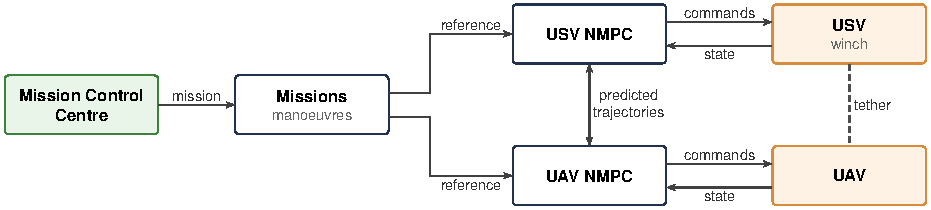
\includegraphics[width=0.62\textwidth]{Introduction/figures/system_overview.pdf}
    \caption{Overview of the system: the missions chain the manoeuvres of both vehicles, which give the references of their NMPCs, and the two controllers exchange their predicted trajectories.}
    \label{fig:overview}
\end{figure*}

\textbf{USV NMPC.} To limit both the thrusts and their rates, the thrusts and angles are included in the state, $\mathbf{x}_v = [x,y,\psi,u,v,r,T_L,T_R,\alpha_L,\alpha_R]^\top$, and the inputs are their rates, bounded by the limits of the thrusters. The stage cost penalises the errors of position, heading and velocity, $\|\mathbf{p}-\mathbf{p}_{ref}\|^2_{Q_p} + q_\psi(1-\cos(\psi-\psi_{ref})) + \|\boldsymbol\nu-\boldsymbol\nu_{ref}\|^2_{Q_\nu}$, together with the thrusts and their rates. A soft lower bound on the surge speed keeps the vessel sailing bow first, and the separation from the predicted trajectory of the UAV, $\hat{\mathbf{p}}_a$, is limited by the reach of the tether,
\begin{equation}
    (x-\hat x_a)^2 + (y-\hat y_a)^2 + (\hat z_a - z_t)^2 - d_{max}^2 \le \sigma,
    \label{eq:usv_tether}
\end{equation}
where $z_t$ is the height of the winch. The USV NMPC runs at $10\,\text{Hz}$ with a horizon of $2\,\text{s}$.

\textbf{UAV NMPC.} The commanded attitude and the thrust are included in the state, $\mathbf{x}_a = [\mathbf{p},\dot{\mathbf{p}},\phi,\theta,\psi,\phi_{\mathrm{cmd}},\theta_{\mathrm{cmd}},\psi_{\mathrm{cmd}},T]^\top$, the inputs are their rates, and the model combines \eqref{eq:uav_dyn}--\eqref{eq:tether_force}, with the tether attached to the predicted trajectory of the USV. The stage cost penalises the errors of position and velocity, the tilt, the deviation of the thrust from hover and the inputs, and keeps the UAV looking at the winch, a term that fades within about $2\,\text{m}$ of it. The soft constraints $h_1$--$h_7$ bound the height, the horizontal and vertical speeds and the tilt, which is applied to both the attitude and its command, $\max(|\phi|,|\phi_{\mathrm{cmd}}|) \le \phi_{max}$, so that the command sent to the autopilot also respects it. The tether gives the last two: the separation is limited, $d^2 \le d_{max}^2$, and so is the rate at which it grows, $\mathbf{r}^\top\dot{\mathbf{r}}/d \le \dot d_{max}$, which may not exceed the pay-out of the winch. The UAV NMPC runs at $50\,\text{Hz}$ with a horizon of $1\,\text{s}$.

\textbf{Disturbance observer.} A force that the model does not describe, such as wind, makes the prediction drift and leaves a steady offset. Following the disturbance-model approach to offset-free predictive control~\cite{pannocchia2003offsetfree,maeder2009offsetfree}, an external force $\hat{\mathbf{F}}_{\mathrm{ext}}$, held constant over the horizon, is added to \eqref{eq:uav_dyn} and estimated from the one-step prediction error of the velocity,
\begin{equation}
    \hat{\mathbf{F}}_{\mathrm{ext},k} = \mathrm{sat}_{\bar F}\Big(\hat{\mathbf{F}}_{\mathrm{ext},k-1} + \beta\frac{m}{T_s}\big(\mathbf{v}_k - \hat{\mathbf{v}}_{k|k-1}\big)\Big),
    \label{eq:observer}
\end{equation}
with a gain $\beta = 0.03$, which gives a time constant of about $T_s/\beta \approx 0.7\,\text{s}$, and a bound $\bar F = 8\,\text{N}$.
